\subsubsection{Comparison with HPC Clusters}

Scientific computing applications are typically run on large-scale HPC clusters, where different performance and cost dynamics apply.
While there are hardware differences between cloud VMs and HPC clusters that can contribute to performance differences, we are interested in the performance ``overheads''.
In the case of \sysname, the job failures and recomputations increase the job turnaround time, and are thus the main source of overhead.

On HPC clusters, jobs enjoy significantly lower recomputation probability, since the hardware on these clusters has MTTFs in the range of years to centuries~\cite{dongarra_fault_nodate}.
However, we emphasize that there exist \emph{other} sources of performance overheads in HPC clusters.
In particular, since HPC clusters have high resource utilization, they also have significant \emph{waiting} times. 
On the other hand, cloud resource utilization is low~\cite{borg} and there is usually no need to wait for resources, which is why transient servers exist in the first place. 


Thus, we compare the performance overhead due to preemptions for \sysname, and job waiting times in conventional HPC deployments.
To obtain the job waiting times in HPC clusters, we use the LANL Mustang traces published as part of the Atlas trace repository~\cite{cmu-atlas}.
We analyze the waiting time of over two million jobs submitted over a 5 year period, and compute the increase in running time of the job due to the job waiting or queuing time. 

\begin{figure}[t]
  \centering 
  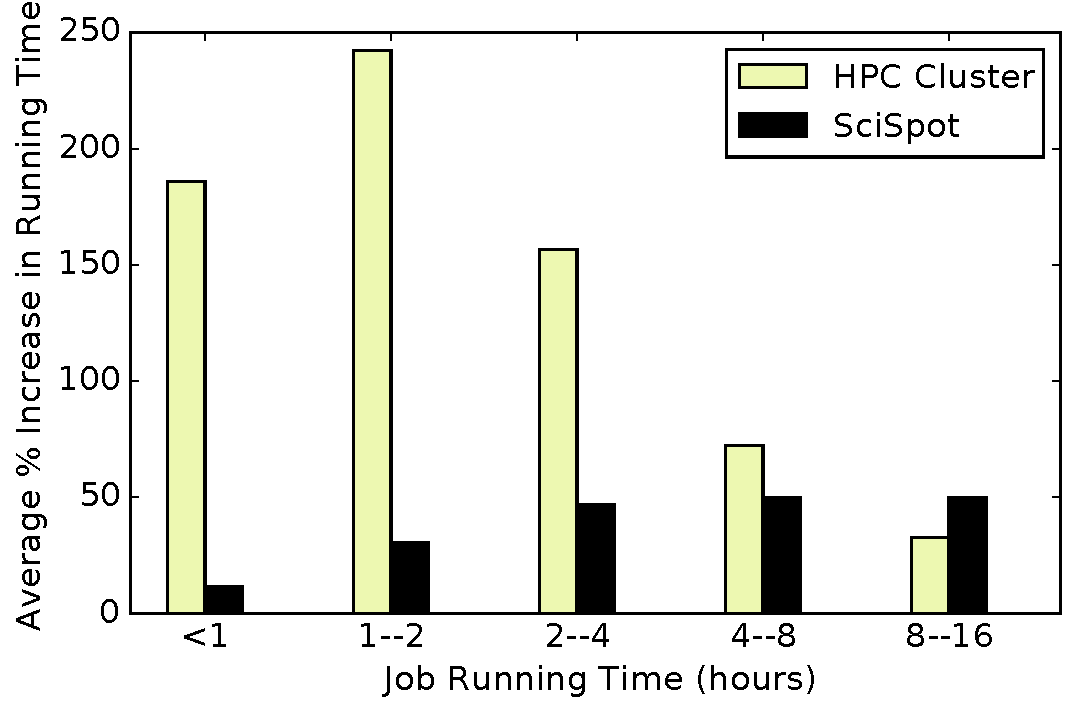
\includegraphics[width=0.4\textwidth]{../graphs/hpc-vs-scispot.pdf}
      \vspace*{\myfigspace}
  \caption{Increase in running time due to waiting on HPC clusters is significantly higher than the recomputation time for \sysname, except for very long and rare jobs (see inset). }
  \label{fig:hpc-vs-scispot}
  \vspace*{\myfigspace}
\end{figure}


%We define the overhead as the increase in running time which is equal to the turnaround time (i.e., the time between the job submission and successful completion) divided by the base job running time (with no waiting or premptions). 
%In HPC clusters, the overhead is the waiting time for resources, and in \sysname the overhead is the recomputation time due to preemptions.
Figure~\ref{fig:hpc-vs-scispot} compares the overhead (as percentage increase in running time) of \sysname and HPC clusters  for jobs of different lengths. We see that the average performance overhead due to waiting can be significant in the case of HPC clusters, and the job submission latency and queuing time dominate for smaller jobs, increasing their total turnaround time by more $2.5\times$.
This waiting is amortized in the case of longer running jobs, and the overhead for longer jobs is around 30\%.

On the other hand, \sysname's performance overhead is significantly smaller for jobs of up to 8 hours in length.
For longer jobs, the limited lifetime of Google Preemptible VMs (24 hours) begins to significantly increase the preemption probability and expected recomputation time.
We emphasize that these are \emph{individual} job lengths, and not the running time of entire bag of jobs.
We note that these large single jobs are rare, accounting for less than 5\% of all HPC jobs (see inset in Figure~\ref{fig:hpc-vs-scispot}).
For smaller jobs (within a much larger bag), both the preemption probability and recomputation overhead is much smaller. 

\noindent \emph{\textbf{Result:} \sysname's overhead of recomputation due to preemptions is small, and is up to $10\times$ lower compared to the overhead of waiting in conventional HPC clusters. }

% \subsubsection{Comparison with HPC Performance}
% The performance of scientific computing applications has been extensively compared on HPC and cloud setups~\cite{iosup_performance_2011, zhai_cloud_2011, marathe2013comparative, galante_analysis_2016, benedictis_cloud-aware_2014}. 
% For completeness, we show the running times on the Big Red II supercomputing cluster in Table~\ref{tab:bigred2}, with 16 CPU nodes used throughout, and we see that our representative applications \emph{do not} face a penalty when deployed on the cloud. 
% 
% % This is confinement/shapes comparison against Big Red II
\begin{table}[]
  \begin{tabular}{|l|l|r|r|}
    \hline
    \# Application & Nodes & Big Red II & \sysname \\
    \hline
  	Nanoconfinement	&	1	&	2370	& 1546	\\
    Nanoconfinement	&	4	&	1140	&	851	\\
    \hline
  	Shapes	&	1	&	2649	& 1194	\\
    Shapes	&	4	&	1209	&	548	\\
    \hline
\end{tabular}
\caption{Running times (in seconds) of different applications on the Big Red II HPC cluster vs \sysname.}
\label{tab:bigred2}
  \vspace*{\myfigspace}
\end{table}




%%%%%%%%%%%%%%%%%%%%%%%%%%%%%%%%%%%%%%%%%%%%%%%%%%%%%%%%%%%%%%%%%%%%%%%%%%%%%%%%

\subsection{SciSpot Scaling}

We now turn our attention to \sysname's scaling properties. We are primarily interested in observing the behavior of running bags of jobs of different applications with different resource requirements.
In all cases unless otherwise stated, we run bags of 36 jobs, and impose that 90\% of all jobs complete (thus we target a completion of 32 jobs).
The jobs in the bags are for exploring the different parameters (i.e., doing a parameter sweep), using \sysname's automated parameter sweeping functionality described in Section~\ref{sec:impl}.
%For reference, the distribution of running times for the different applications is shown in Figure~\ref{fig:job-run-cdf}. 
In the rest of this section, we evaluate \sysname with different cluster  sizes, number of preemptions, and bag sizes. 

% \begin{figure}
%   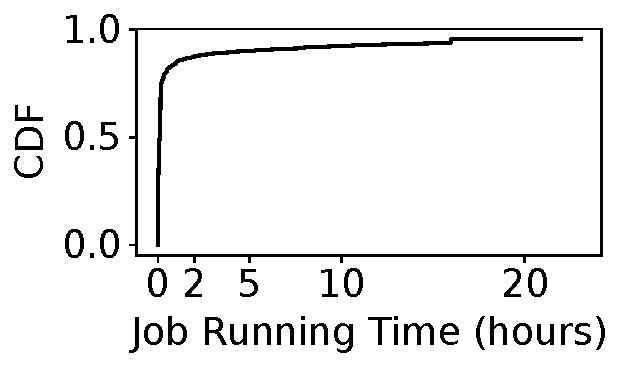
\includegraphics[width=0.2\textwidth]{../graphs/job-run-cdf.pdf}
%   \vspace*{\myfigspace}
%   \caption{Most HPC jobs are less than 2 hours.}
%   \label{fig:job-run-cdf}
%     \vspace*{\myfigspace}
% \end{figure}

%%%%%%%%%%%%%%%%%%%%%%%%%%%%%%%%%%%%%%%%%%%%%%%%%%
%\vspace*{\subsecspace}


\subsubsection{Increasing Cluster Size} 

\begin{figure}
  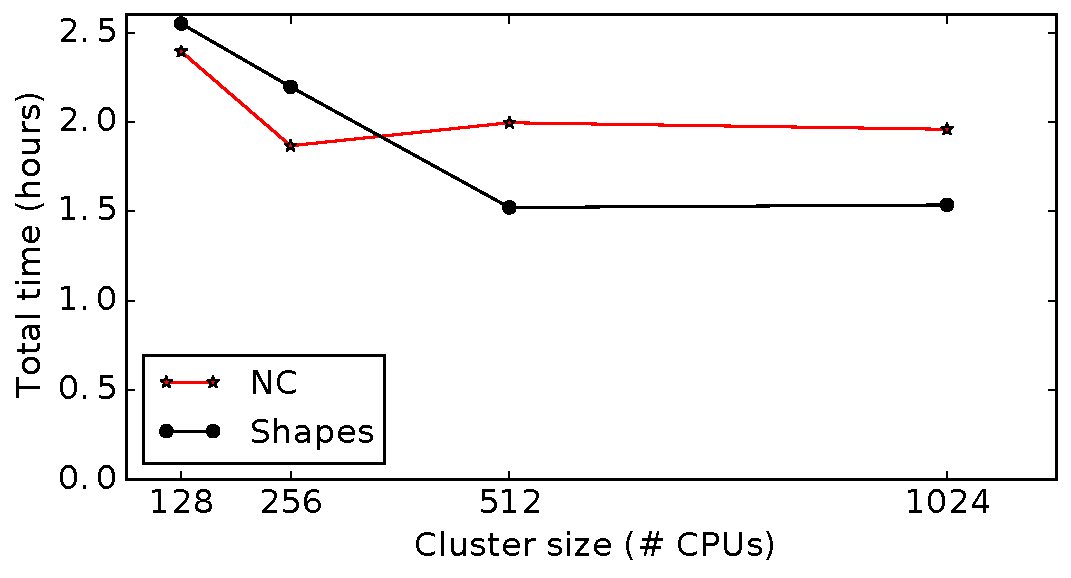
\includegraphics[width=0.4\textwidth]{../graphs/vm-per-job-scaling.pdf}
      \vspace*{\myfigspace}
  \caption{Bag of jobs running times exhibit classic parallel scaling behavior---performance improves until reaching a saturation point.}
  \label{fig:vm-per-job-scaling}
    \vspace*{\myfigspace}
\end{figure}

It is common to deploy scientific computing applications on large clusters, and we evaluate \sysname on different cluster sizes in Figure~\ref{fig:vm-per-job-scaling}.
The figure shows the total running time (i.e., turnaround time) of the bag of jobs for the Nanoconfinement and Shapes applications as the total number of VMs (and hence total number of CPUs) increases.
The error bars in Figure~\ref{fig:vm-per-job-scaling} indicate the running times of individual jobs in the bag. 
For this experiment, we used \texttt{n1-highcpu-32} VMs with 32 CPUs each, and we ran four jobs in parallel on the entire cluster. 
We see classic scaling behavior: both applications can scale to a higher number of VMs up to a point, after which communication overhead  dominates, the performance saturates, and we see no reduction in running time. 


%%%%%%%%%%%%%%%%%%%%%%%%%%%%%%%%%%%%%%%%%%%%%%%%%%
\subsubsection{Increasing Bag Size}

We now evaluate \sysname's behavior when running larger bags of jobs.
Table~\ref{tab:100-jobs} shows the total running time of bags of 32 and 100 jobs.
Since \sysname reuses VMs when running jobs from a bag, it is able to take advantage of the relatively low preemption rates of VMs once they pass the first phase of early failures (Figure~\ref{fig:gcp1}), and thus minimizes the number of preemptions as well as job failures. 
This makes \sysname particularly suitable for running the large bags of jobs that are required when using machine learning techniques for HPC workloads~\cite{ml.atomic2017,melko2017,sam2017,fu2017,long2015machine,ferguson2017machine,ward2018matminer,jcs2,fox2019learning}, since the training and testing data needed for statistical machine learning can be generated using \sysname's bag of jobs. 


%32_2_4 
\begin{table}
  \begin{tabular}{|l|r|r|r|}
    \hline
    Application & Jobs & Time (Hours) & \# Preemptions \\
    \hline
    Nanoconfinement & 32  & 1.87 & 0 \\
     & 100  & 6.08 & 1 \\
    \hline
    Shapes & 32 & 1.47 & 0 \\
     & 100 & 4.49 & 5  \\  
    \hline
  \end{tabular}
  \caption{Running times and number of preemptions for bags of different sizes. }
  \label{tab:100-jobs}
  \vspace*{\myfigspace}
  \vspace*{\myfigspace}
\end{table}



%%%%%%%%%%%%%%%%%%%%%%%%%%%%%%%%%%%%%%%%%%%%%%%%%%
\subsubsection{Increasing Preemptions}

By reusing VMs across a bag of jobs and taking advantage of the low preemption rates during the middle of the 24 hour life of the preemptible VMs, the \emph{expected} job failure rates and recomputation times are fairly small with \sysname (as shown in Figures~\ref{fig:runtimes-bar},~\ref{fig:hpc-vs-scispot}).
However, preemption rates can increase when the cloud operator sees high demand for resources.
Figure~\ref{fig:fails-time} shows the running time of the bag of 32 Nanoconfinement jobs on a cluster of 4 \texttt{n1-highcpu-32} VMs, when different number of VMs are preempted. 
%
We see that even with a high number of preemptions, the running time only increases by 50\%.
This is because most job failures are due to early VM preemptions, as observed in our empirical and analytical models, and this reduces the recomputation time. 
We note that a higher than expected preemption rate (as shown in the figure) is rare, and happens with a vanishingly small likelihood. 
This shows that \sysname is robust and can provide acceptable performance even under extreme, adverse conditions. 


%Summary of results? 

%%%%%%%%%%%%%%%%%%%%%%%%%%%%%%%%%%%%%%%%%%%%%%%%%%


%%% Local Variables:
%%% mode: latex
%%% TeX-master: "paper"
%%% End:
